The techniques we have developed to perform fast computations in some
finite-dimensional algebras, find an application in some
number-theoretic computations on elliptic curves.

\pdfmctwo{Added François' paper}
Elliptic curves are a central object of study in number theory and
algebraic geometry. They are probably most famous for having being
used by Wiles~\cite{wiles95,wiles+taylor95} to prove of Fermat's last
theorem. In computer science, they have applications in
cryptography~\cite{koblitz87,miller86,blake+seroussi+smart},
factorization~\cite{lenstra87,atkin+morain93,bernstein+birkner+lange+peters08-2}
and primality proving~\cite{atkin+morain93:2,morain07}.

In this section we recall the basic definitions and properties of
elliptic curves, the material is drawn from
\cite{silverman:elliptic,milne1996elliptic,connell:elliptic}.


\section{Definitions}
\label{sec:definitions}

We let $\K$ be a field and $\clot{\K}$ be its algebraic
closure. \index{elliptic~curve}Elliptic curves are genus $1$ curves
over $\clot{\K}$ with a distinguished point.

\subsection{Weierstrass equations}
\label{sec:weierstr-equat}

\begin{definition}[Weierstrass equation]
  \index{Weierstrass~equation} Any elliptic curve $E$ can be viewed as
  the projective variety associated to the equation
  \begin{equation}
    \label{eq:107}
    E\;:\; Y^2Z + a_1XYZ + a_3YZ^2 = X^3 + a_2X^2Z + a_4XZ^2 + a_6Z^3
    \text{,}
  \end{equation}
  with $a_1,\ldots,a_6\in\clot{\K}$.  The distinguished point is
  $[0:1:0]$, called the \index{point~at~infinity}\emph{point at
    infinity} and denoted by $\0$\nomenclature[O]{$\0$}{Point at
    infinity of an elliptic curve}.  When $a_1,\ldots,a_6\in\K$, the
  curve is said to be \emph{defined over $\K$}.
\end{definition}

Eq.~\eqref{eq:107} is called the \emph{homogeneous Weierstrass
  form}\index{Weierstrass~form!homogeneous} of the curve $E$.  After
the change of variables $x=\frac{X}{Z},y=\frac{Y}{Z}$,
Eq.~\eqref{eq:107} can be rewritten as
\begin{equation}
  \label{eq:112}
  E\;:\;y^2 + a_1xy + a_3y = x^3 + a_2x^2 + a_4x + a_6
  \text{,}
\end{equation}
called the \emph{affine Weierstrass
  form}\index{Weierstrass~form!affine}. Then the curve $E$ is the
locus of zeros of Eq.~\eqref{eq:112} in $\clot{\K}^2$ (or, more
exactly, in the affine plane $\mathbb{A}^2$), plus the extra point at
infinity $\0$.

The \index{discriminant~of~an~elliptic~curve}discriminant of
Eq.~\eqref{eq:112} is
\begin{equation}
  \label{eq:118}
  \Delta_E = -b_2^2b_8-8b_4^3-27b_6^2+9b_2b_4b_6
  \text{,}
\end{equation}
where
\begin{equation}
  \label{eq:117}
  \begin{aligned}
    b_2 &= a_1^2 + 4a_2\text{,}\\
    b_4 &= 2a_4 + a_1a_3\text{,}\\
    b_6 &= a_3^2 + 4a_6\text{,}\\
    b_8 &= a_1^2a_6+4a_2a_6-a_1a_3a_4+a_2a_3^2-a_4^2\text{.}
  \end{aligned}
\end{equation}

\begin{remark}
  The curve defined by~\eqref{eq:112} has an unique singular point if
  and only if $\Delta_E=0$.  Figure~\ref{fig:singular} shows the two
  possible shapes of a singular curve over the reals. Then, every line
  passing through the singular point meets the curve in another unique
  point. This parameterization makes $E$ birationally equivalent to
  $\Proj^1$, thus $E$ has genus $0$. The converse is also true, thus
  Eq.~\eqref{eq:112} defines an elliptic curve if and only if
  $\Delta_E\ne0$.
\end{remark}


\begin{figure}[ht]
  \centering
  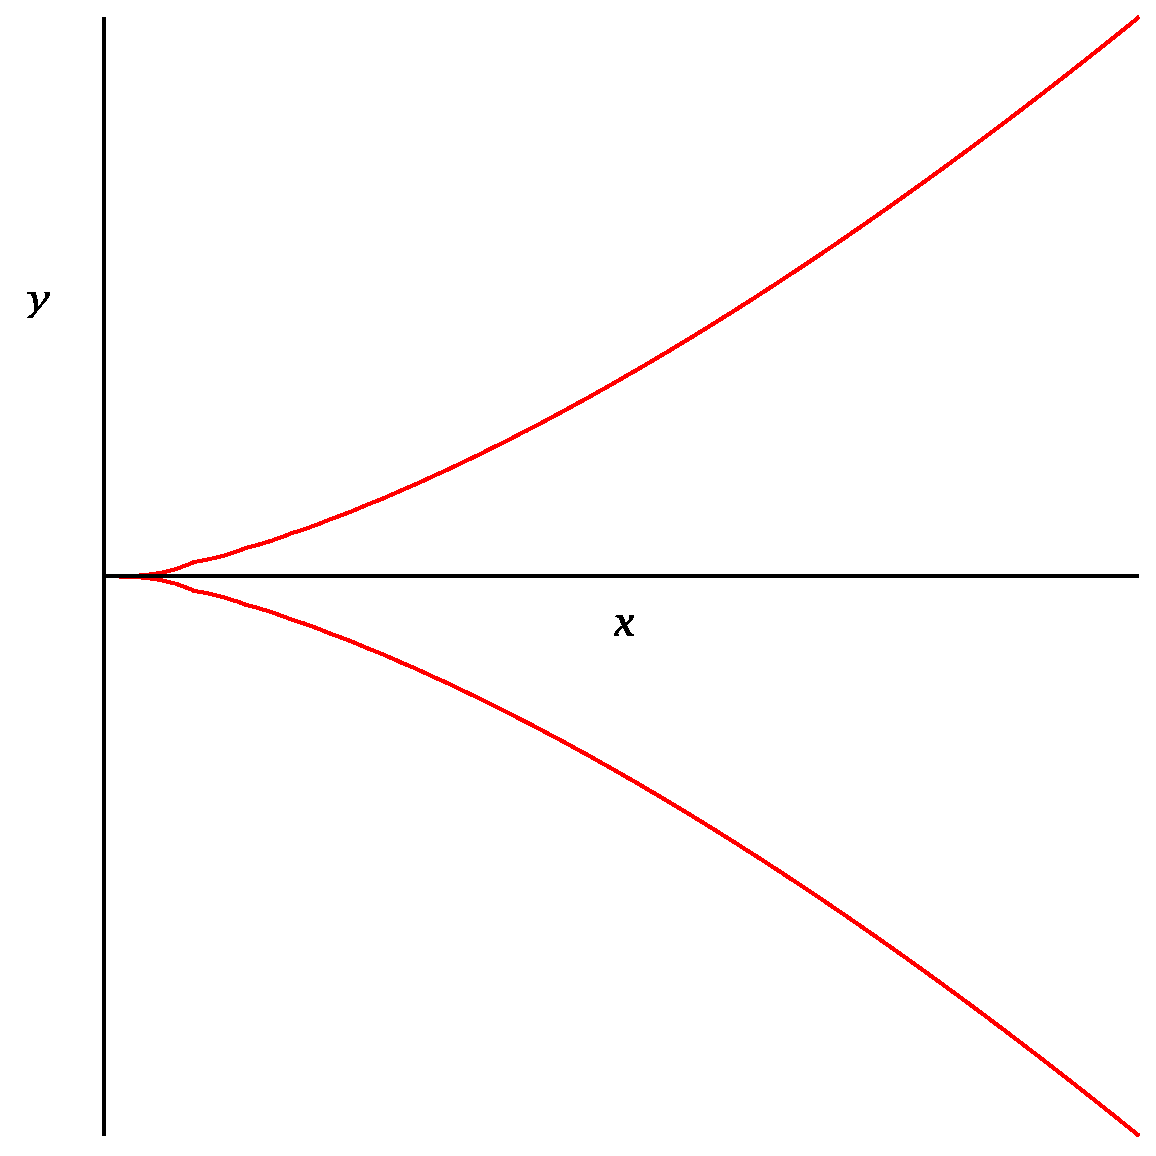
\includegraphics[width=0.45\textwidth]{isogeny/cusp}
  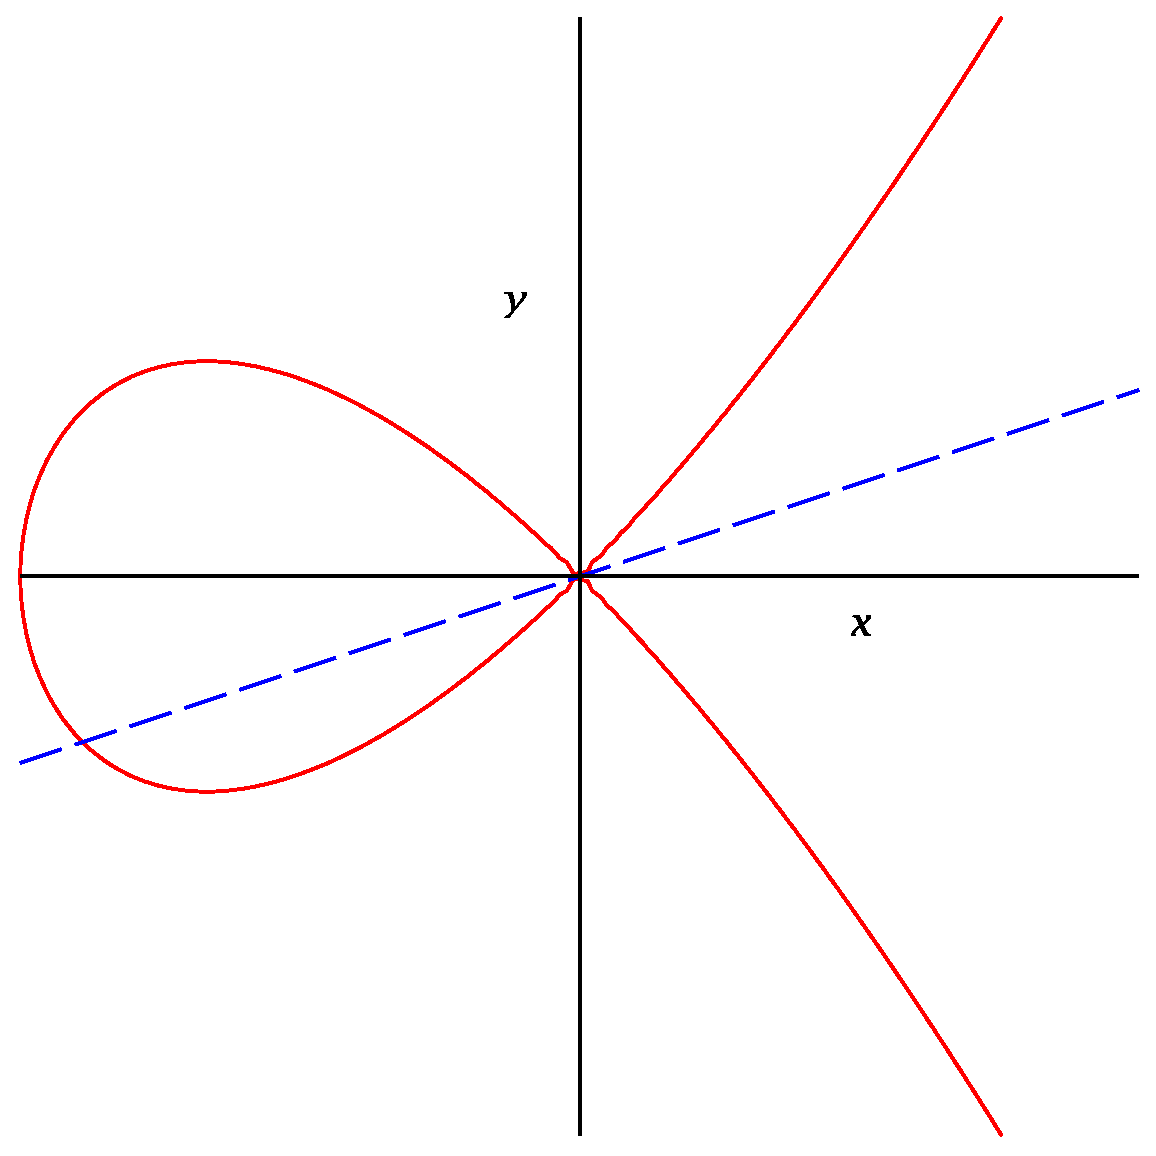
\includegraphics[width=0.45\textwidth]{isogeny/node}
  \caption{Two singular Weierstrass curves. On the left $y^2=x^3$, on
    the right $y^2=x^3+x^2$. On the right we have shown the
    parameterization by the line passing through the origin.}
  \label{fig:singular}
\end{figure}

\begin{definition}[$j$-invariant]
  \index{j-invariant@$j$-invariant}%
  \nomenclature[j]{$j_E$}{$j$-invariant of an elliptic curve $E$}
  We associate to the curve $E$ defined by Eq.~\eqref{eq:112}, the
  $j$-invariant
 \[j_E = \frac{(b_2^2-24b_4)^3}{\Delta_E}\text{.}\]
\end{definition}

\begin{nota}
  Recall that if $E$ is an elliptic curve defined by an affine
  Weierstrass equation $f(x,y)=0$ with coefficients in $\K$, its
  \hyperref[sec:algebraic-varieties]{function field} $\K(E)$ is the
  field of fractions of
  \begin{equation}
    \label{eq:125}
    \K[E]\eqdef\K[x,y]/(f(x,y))
    \text{.}
  \end{equation}
\end{nota}


\subsection{Group law}
\label{sec:group-law}
\pdfmctwo{I find both "chord-tangent"
  and "chord and tangent" in the literature.}  Elliptic curves are
endowed with a group structure via the
\index{elliptic~curve!group~law}
\index{chord-tangent~law}\emph{chord-tangent law}.

\begin{definition}
  \pdfmctwo{Yes, P2 has been (quickly) defined in Chap 1.}
  Let $E$ be an elliptic curve and let $P,Q\in\Proj^2$ be two points
  on the curve. Let $L$ be the line passing through $P$ and $Q$, with
  multiplicity two if $P=Q$, and let $R$ be the third intersection
  point with $E$.  Let $L'$ be the line passing through $R$ and
  $\0$. Then the point $P+Q$ is defined as the third point of
  intersection of $L'$ and $E$.
\end{definition}

\begin{figure}[ht]
  \centering
  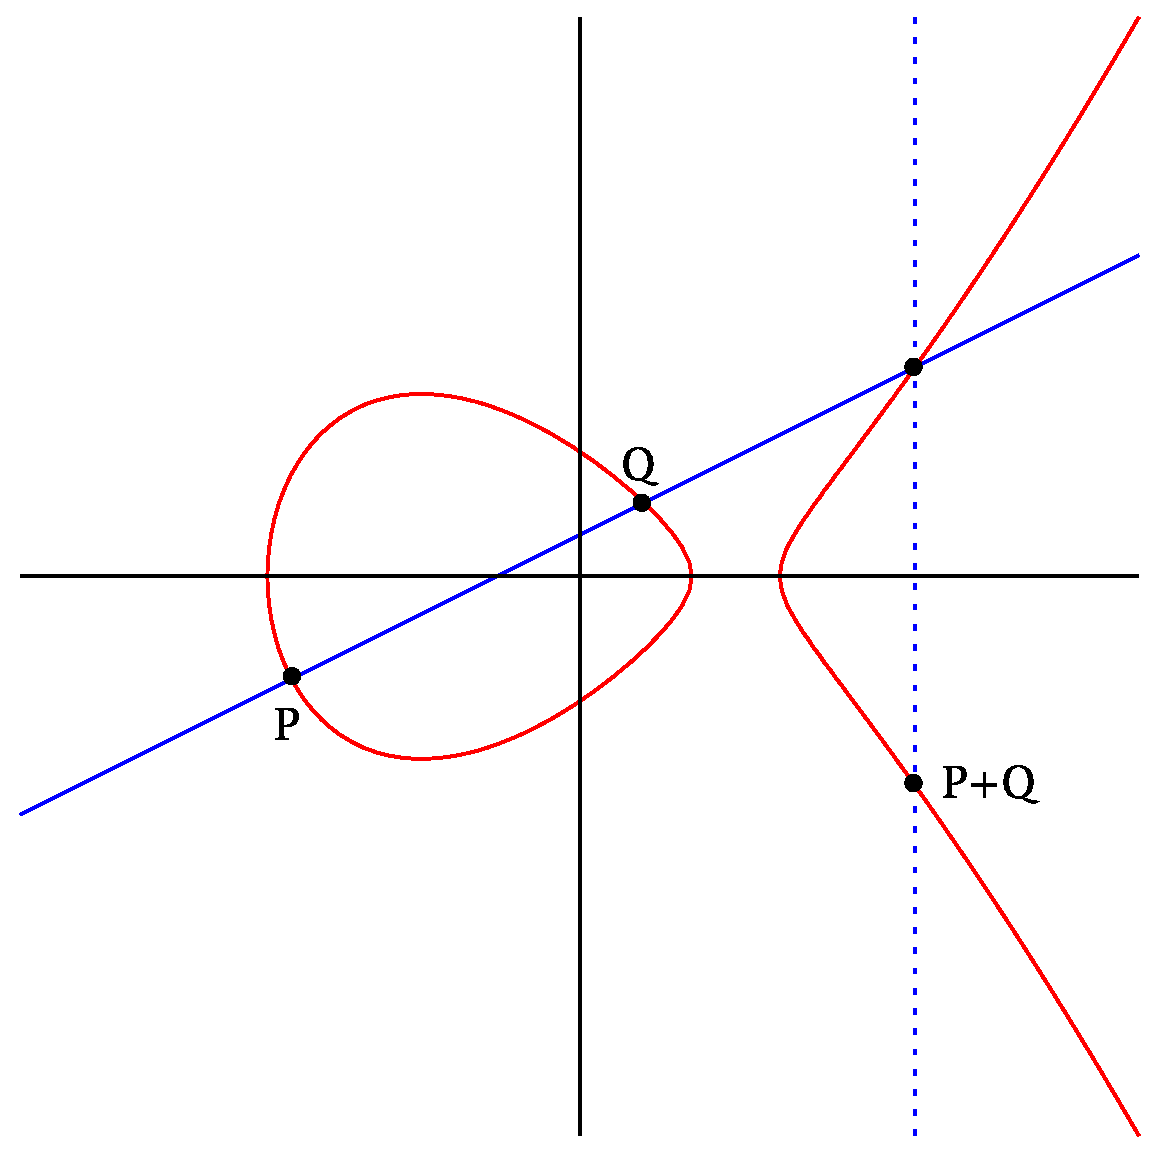
\includegraphics[width=0.5\textwidth]{isogeny/ec-add}
  \caption{Chord-tangent law on an elliptic curve defined over the reals.}
  \label{fig:chord-tangent}
\end{figure}

The definition is pictured in Figure~\ref{fig:chord-tangent}. For a
proof that this defines indeed a group law on the points of $E$, with
$\0$ being the identity element, see \cite[II, $\S2$]{silverman:elliptic}.

\begin{definition}[Rational points]%
  \nomenclature[E]{$E(\K)$}{Set of $\K$-rational points of an elliptic curve $E$}
  Let $E$ be an elliptic curve defined over $\K$, the set of
  \emph{$\K$-rational points}\index{rational~point} $E(\K)$ is 
  \begin{equation}
    \label{eq:119}
    E(\K) = E \cap \Proj^2(\K)
    \text{.}
  \end{equation}
\end{definition}

If $P$ and $Q$ are rational points, the lines $L$ and $L'$ are defined
by equations over $\K$, thus $E(\K)$ forms a subgroup of $E$. To allow
calculations in $E(\K)$ without having to lift the coefficients in an
algebraic closure, it is convenient to give explicit formulas for the
chord-tangent law. 

We shall give the formulas for affine coordinates. $x,y$ are functions
in $\K(E)$, thus from now on, if $P$ is a point of $E$, we denote by
$x(P)$ its abscissa and by $y(P)$ its ordinate (in affine coordinates).

\begin{proposition}
  Let $E$ be the elliptic curve defined by Eq.~\eqref{eq:112}. Let
  $P$, be a point of $E$ different from $\0$, the coordinates of $-P$
  are given by
  \begin{equation}
    \label{eq:120}
    x(-P) = x(P)\text{,}\qquad y(-P)=-y(P) -a_1x(P) - a_3
    \text{.}
  \end{equation}
  Let $P,Q$ be points of $E$ different from $\0$ and let $Q\ne-P$, the
  coordinates of $P+Q$ are given by
  \begin{equation}
    \label{eq:121}
    \begin{aligned}
      \lambda &= \begin{cases}
        \frac{y(Q) - y(P)}{x(Q) -x(P)} &\text{if $P\ne Q$,}\\
        \frac{3x(P)^2+2a_2x(P)+a_4-a_1y(P)}{2y(P)+a_1x(P)+a_3} &\text{if $P=Q$,}
      \end{cases}\\
      x(P+Q) &= \lambda^2+a_1\lambda-a_2-x(P)-x(Q)\text{,}\\
      y(P+Q) &= -(\lambda+a_1)x(P+Q) - y(P) + \lambda x(P)-a_3\text{.}
    \end{aligned}
  \end{equation}
\end{proposition}

For $m\in\Z$, we denote by $[m]P$ the point%
\nomenclature[mP]{$[m]P$}{Scalar multiple of a point of an elliptic
  curve} $\overbrace{P+P+\cdots+P}^{m\text{ times}}$ if $m>0$, or the
point $[-m](-P)$ if $m<0$, or $\0$ if $m=0$. 

\begin{definition}[Kummer variety]
  \pdfmcone{Oups! Changed "Kummer surface" to "Kummer variety"
    (it is called "surface" only for two-dimensional abelian varieties).}
  \label{def:kummer}
  The \index{Kummer~variety}\emph{Kummer variety} of an elliptic curve
  $E$, denoted by $K_E$\nomenclature[KE]{$K_E$}{Kummer variety of an
    elliptic curve}, is the quotient of $E$ by the equivalence
  relation $P\simeq-P$.
\end{definition}

\begin{remark}
  \label{rk:montgomery}
  The Kummer variety can be represented by taking the abscissas of the
  points of $E$. It is not a group, but we can still compute scalar
  multiples of its points. In fact, from the addition formulas we
  deduce for $P\ne-P$
  \begin{equation}
    \label{eq:128}
    x([2]P) = \frac{x^4-b_4x^2-2b_6x-b_8}{4x^3+b_2x^2+2b_4x+b_6}
    \text{,}
  \end{equation}
  where $x=x(P)$; and for $P\ne Q$
  \begin{equation}
    \label{eq:129}
    x(P+Q) + x(P-Q) =
    \frac{2\pi\sigma + b_2\pi + b_4\sigma + b_6}{(x(P)-x(Q))^2}
    \text{,}
  \end{equation}
  where $\pi=x(P)x(Q)$ and $\sigma=x(P)+x(Q)$. 

  Then, to compute $x([n]P)$, we start from $x(P)$ and $x([2]P)$, and
  we iteratively apply
  \begin{equation}
    \label{eq:130}
    \begin{aligned}[]
      [2i]P   &= [2][i]P\text{,}\\
      [2i+1]P &= [i+1]P + [i]P\text{,}
    \end{aligned}
  \end{equation}  
  or
  \begin{equation}
    \label{eq:131}
    \begin{aligned}[]
      [2i+1]P &= [i+1]P + [i]P\text{,}\\
      [2i+2]P &= [2][i+1]P\text{,}
    \end{aligned}
  \end{equation}
  until we reach $[n]P$. This algorithm appeared
  in~\cite{montgomery87} and is sometimes referred to as
  \index{Montgomery's formulas}\emph{Montgomery's formulas}.
\end{remark}

The map
\begin{equation}
  \label{eq:122}
  \begin{aligned}[]
    [m]_E : E(\K) &\ra E(\K)\text{,}\\
    P &\mapsto [m]P
  \end{aligned}
\end{equation}
is a group endomorphisms of $E(\K)$. 

\begin{definition}
  The $m$-th \emph{torsion subgroup} of $E$ is
  \begin{equation}
    \label{eq:123}
    E[m] = \{P\in E(\clot{\K}) \,|\, [m]P=\0\}
    \text{,}
  \end{equation}
  its points are called%
  \nomenclature[E]{$E[m]$}{$m$-torsion subgroup of an elliptic curve
    $E$}
  \index{elliptic~curve!torsion~subgroup}\index{torsion~point}\emph{$m$-torsion
    points}.
\end{definition}

Since addition is an algebraic map, multiplication by $n$ is algebraic
too. It can be shown that there exist polynomials
$\psi_m,\theta_m,\omega_m\in\K(E)$ such that
\begin{equation}
  \label{eq:124}
  [m](x,y) = \left(\frac{\theta_m(x,y)}{\psi_m(x,y)^2},
    \frac{\omega_m(x,y)}{\psi_m(x,y)^3}\right)
  \text{.}
\end{equation}

\begin{definition}[Division polynomials]
  The polynomial $\psi_m$ is called the
  \index{division~polynomial}\emph{$m$-th division polynomial}.
\end{definition}

\begin{remark}
  The division polynomials can be computed from the addition formulas
  via a double-and-add approach. Their importance comes from the fact
  that $\psi_m$ vanishes on $E[m]$.
\end{remark}

From the formulas for the division polynomials one can deduce the
structure of the $m$-torsion.

\begin{theorem}
  Let $p$ be the characteristic of $\K$. If $p$ does not divide $m$
  \begin{equation}
    \label{eq:126}
    E[m] \isom \Z/m\Z\times\Z/m\Z
    \text{;}
  \end{equation}
  if $p\ne0$, then for every $i>0$ either
  \begin{equation}
    \label{eq:127}
    E[p^i] = \{\0\}\text{,} 
    \qquad\text{or}\qquad E[p^i] \isom \Z/p^i\Z
    \text{.}
  \end{equation}
\end{theorem}

\begin{definition}[Supersingular, ordinary]
  An elliptic curve $E$ is said to be
  \index{elliptic~curve!supersingular}\index{supersingular}\emph{supersingular}
  if $E[p^i]=\{\0\}$ for any $i$; it is said to be
  \index{elliptic~curve!ordinary}\emph{ordinary} otherwise.
\end{definition}

\begin{definition}[Tate module]
  Let $\ell$ be a prime, the \index{Tate~module}\emph{$\ell$-adic Tate
    module}
  $\mathcal{T}_\ell(E)$\nomenclature[Tl]{$\mathcal{T}_\ell(E)$}{$\ell$-adic
    Tate module} is the group
  \begin{equation}
    \label{eq:132}
    \mathcal{T}_\ell(E) = \varprojlim_n E[\ell^n]
  \end{equation}
  with respect to the projections
  \begin{equation}
    \label{eq:133}
    [\ell]_E : E[\ell^{n+1}] \ra E[\ell^{n}]
    \text{.}
  \end{equation}
\end{definition}

\begin{proposition}
  The Tate module has a natural structure of
  $\Z_\ell$-module\nomenclature*[Zp]{$\Z_p$}{$p$-adic integers}. As
  such
  \begin{equation}
    \label{eq:134}
    \mathcal{T}_\ell(E) \isom
    \begin{cases}
      \Z_\ell\times\Z_\ell &\text{if $\ell\ne p$,}\\
      \Z_p &\text{if $\ell=\car(\K)$ and $E$ is ordinary,}\\
      \{\0\} &\text{if $E$ is supersingular.}
    \end{cases}
  \end{equation}
\end{proposition}


\subsection{Isomorphisms}
\label{sec:isomorphisms}

Let $E$ and $E'$ be two elliptic curves in Weierstrass form over a
field $\K$, they are said to be isomorphic if there is a linear change
of variables that transforms one equation in the other and preserves
the point at infinity.  Then, clearly $E(\clot{\K})$ and
$E'(\clot{\K})$ are isomorphic as groups. If the change of variables
has coefficients in $\K$, the curves are said to be
\index{isomorphism!of~elliptic~curves}\index{elliptic~curve!isomorphic}isomorphic
over $\K$, then $E(\K)$ and $E'(\K)$ are isomorphic as groups.

It can be shown that the only such changes of variables are
\begin{equation}
  \label{eq:116}
  \begin{aligned}
    x &= u^2x' + r\text{,}\\
    y &= u^3y' + u^2sx' + t\text{,}
  \end{aligned}
\end{equation}
with $r,s,t,u\in\clot{\K}$ and $u\ne0$.

\begin{proposition}
  Two elliptic curves $E$ and $E'$ in Weierstrass form are isomorphic
  over $\clot{\K}$ if and only if $j_E=j_{E'}$.
\end{proposition}

\index{Weierstrass~form!simplified~form}Weierstrass equations can be
brought via isomorphism to a form that is easier to handle, called
\emph{simplified Weierstrass form}. The following classification is
from~\cite{connell:elliptic}.

\begin{proposition}[Simplified Weierstrass form]
  \label{th:simplified-weierstrass}
  Any elliptic curve is isomorphic to one of the following Weierstrass
  forms:
  \begin{itemize}
  \item If $\car(\K)=0$ or $\car(\K)>3$
    \begin{equation}
      \label{eq:weierstrass>3}
      E\;:\;y^2 = x^3 + ax + b 
      \qquad\text{and}\qquad
      j_E = \frac{1728(4a)^3}{16(4a^3 + 27b^2)}
      \text{;}
    \end{equation}
  \item if $\car(\K)=3$ and $E$ is ordinary
    \begin{equation}
      \label{eq:weierstrass=3}
      E\;:\;y^2 = x^3 + ax^2 + b
      \qquad\text{and}\qquad
      j_E = -\frac{a^3}{b}
      \text{;}
    \end{equation}
  \item if $\car(\K)=3$ and $E$ is supersingular
    \begin{equation}
      \label{eq:136}
      E\;:\;y^2=x^3 + ax+b
      \qquad\text{and}\qquad
      j_E=0
      \text{;}
    \end{equation}
  \item if $\car(\K)=2$ and $E$ is ordinary
    \begin{equation}
      \label{eq:weierstrass=2}
      y^2 + xy = x^3 + ax^2 + b
      \qquad\text{and}\qquad
      j_E = \frac{1}{b}
      \text{;}
    \end{equation}
  \item if $\car(\K)=2$ and $E$ is supersingular
    \begin{equation}
      \label{eq:137}
      E\;:\; y^2 + a_3y = x^3 + a_4x + a_6
      \qquad\text{and}\qquad
      j_E = 0
      \text{.}
    \end{equation}
  \end{itemize}
\end{proposition}

\begin{definition}[Twist]
  Two non-isomorphic elliptic curves $E$ and $E'$ over $\K$ such that
  $j_E=j_{E'}$ are called \index{twist}\emph{twists} (of one another).
\end{definition}

\pdfmctwo{I was following Connell on the terminology about twists. I
  changed the terminology, hope that it is more standard now.}  An
elliptic curve and a twist are isomorphic over the algebraic closure
$\clot{\K}$. The \index{twist!degree~of~a}degree of a twist is the
degree of the smallest extension $\K'/\K$ such that the two curves are
isomorphic over $\K'$.

\begin{proposition}
  Any curve has a quadratic twist. Any twist of an ordinary elliptic
  curve is quadratic.
\end{proposition}


\subsection{Isogenies}
\label{sec:isogenies}

\begin{definition}[Isogeny]
  Let $E$ and $E'$ be elliptic curves, an
  \index{isogeny}\emph{isogeny} $E\ra E$ is a morphism of varieties
  that preserves the point at infinity.
\end{definition}

It turns out that isogenies preserve the group structure.

\begin{theorem}
  Let $\I:E\ra E'$ be an isogeny, then it is a group morphism
  $E(\clot{\K})\ra E'(\clot{\K})$. It is surjective and its kernel is
  finite. Furthermore, if $\I$ is defined over $\K$, then its
  restriction to $E(\K)$ is a group morphism $E(\K)\ra E'(\K)$.
\end{theorem}

\begin{definition}[Degree]
  Let $\I$ be an isogeny and
  \index{degree!of~an~isogeny}\index{isogeny!degree}define
  \begin{equation}
    \label{eq:138}
    \begin{aligned}
      \dual{\I}:\clot{\K}(E')&\ra\clot{\K}(E)\\
      f &\ra f\circ\I
      \text{.}
    \end{aligned}
  \end{equation}
  The \emph{separable (resp. inseparable) degree} of $\I$, denoted by
  $\deg_s\I$ (resp. $\deg_i\I$), is the separable (resp. inseparable)
  degree of the field extension $\clot{\K}(E)/\I(\clot{\K}(E'))$. The
  \emph{degree} of $\I$ is $\deg\I=\deg_s\I\deg_i\I$.

  An isogeny is called \index{isogeny!separable}\emph{separable} if
  $\deg_i\I=1$, \index{isogeny!inseparable}\emph{inseparable}
  otherwise. It is called
  \index{isogeny!purely~inseparable}\emph{purely inseparable} if
  $\deg_s=1$.
\end{definition}

\begin{theorem}
  Let $\I$ be an isogeny, its kernel contains $\deg_s\I$ elements.
\end{theorem}

Two curves are said to be isogenous if there is an isogeny between
them; $\ell$-isogenous if it has degree $\ell$.

One example of isogeny is the map $[m]$, it is a separable isogeny of
degree $m^2$. If $\K$ has characteristic $p$, then the map
\begin{equation}
  \label{eq:139}
  \frobisog : (x,y) \mapsto (x^p,y^p)
\end{equation}
is a purely inseparable isogeny of degree $p$, called the
\index{Frobenius~isogeny}\emph{Frobenius
  isogeny}\nomenclature[f]{$\frobisog$}{Frobenius isogeny:
  $(x,y)\mapsto(x^p,y^p)$}. If $\K$ is a perfect field, any purely
inseparable isogeny is a power of $\frobisog$.

\begin{theorem}
  Any isogeny can be factored into a product of a separable and a
  purely inseparable isogeny.
\end{theorem}

One important property about isogenies is that they factor the
multiplication by $m$ map.

\begin{definition}[Dual isogeny]
  Let $\I : E \rightarrow E'$ be a degree $m$ isogeny. There exists an
  unique isogeny $\hat{\I} : E' \rightarrow E$, called the
  \index{dual~isogeny}\index{isogeny!dual}\emph{dual isogeny} such
  that
  \[\I\circ\hat{\I} = [m]_E \qquad\text{and}\qquad \hat{\I}\circ\I =
  [m]_{E'}\]
\end{definition}

By endomorphism we mean an isogeny $E\ra E$. The multiplication maps
are endomorphisms, thus $\End(E)$ contains a copy of $\Z$.  The main
theorem about the endomorphism ring $\End(E)$ is the following.

\begin{theorem}
  The endomorphism ring is either isomorphic to $\Z$, or to an order
  in a quadratic imaginary field, or to an order in a quaternion
  algebra.
\end{theorem}

If $\car(\K)\ne0$, we can exclude the case $\Z$, because $\End(E)$
contains the Frobenius isogeny. Furthermore, in the two cases
\begin{itemize}
\item $\car(\K)=0$,
\item $\K$ perfect and $E$ ordinary
\end{itemize}
$\End(E)$ cannot be an order in a quaternion algebra, thus it is
commutative.


\section{Curves over \texorpdfstring{$\C$}{C}}
\label{sec:curves-over-c}
Elliptic curves defined over $\C$ have a very simple structure.

\begin{definition}[Lattice]
  A \index{lattice}\emph{lattice} $\Lambda\subset\C$ is a discrete
  additive subgroup of $\C$ that contains a basis of the $\R$-vector
  space $\C$. Two lattices $\Lambda_1,\Lambda_2$ are said to be
  \emph{homothetic} if $\Lambda_1=\alpha\Lambda_2$ for some
  $\alpha\in\C^{\ast}$.
\end{definition}

As a group, a lattice is isomorphic to $\Z\times\Z$. Two elements
$\omega_1,\omega_2\in\Lambda$ such that
\begin{equation}
  \label{eq:135}
  \Lambda = \omega_1\Z + \omega_2\Z
\end{equation}
are called a \emph{basis} of $\Lambda$. The quotient $\C/\Lambda$ is
called a \index{complex torus}\emph{complex torus}.

\begin{definition}[Elliptic function]
  Let $\Lambda$ be a lattice. An
  \index{elliptic~function}\emph{elliptic function} on $\Lambda$ is a
  meromorphic function $f$ on $\C$ such that
  \begin{equation}
    \label{eq:141}
    f(z+\omega) = f(z)
  \end{equation}
  for any $\omega\in\Lambda$.  The set of elliptic functions on
  $\Lambda$ is denoted by $\C(\Lambda)$.
\end{definition}

An example of elliptic function is the
\index{Weierstrass~function@Weierstrass~$\wp$-function}\emph{Weierstrass
  $\wp$-function}\nomenclature[p]{$\wp$}{Weierstrass $\wp$-function}
\begin{equation}
  \label{eq:142}
  \wp(z;\Lambda) = \frac{1}{z^2} + \sum_{\omega\in\Lambda\diffset\{0\}}\frac{1}{(z-\omega)^2}-\frac{1}{\omega^2}
  \text{,}
\end{equation}
\begin{theorem}
  Let $\Lambda$ be a lattice, then $\C(\Lambda) = \C(\wp(z),\wp'(z))$.
\end{theorem}

For $k>1$, we define the \index{Eisenstein~series}\emph{Eisenstein
  series} $G_{2k}$\nomenclature[G2k]{$G_{2k}$}{Eisenstein series} as
\begin{equation}
  \label{eq:143}
  G_{2k}(\Lambda) = \sum_{\omega\in\Lambda\diffset\{0\}}\frac{1}{\omega^2}
  \text{.}
\end{equation}

\begin{theorem}
  The Laurent series expansion of $\wp(z)$ at $0$ is
  \begin{equation}
    \label{eq:144}
    \wp(z) = \frac{1}{z^2} + \sum_{k=1}^\infty (2k+1)G_{2k+2}z^{2k}
    \text{.}
  \end{equation}
  At any $z\not\in\Lambda$, the function $\wp(z)$ satisfies the
  differential equation
  \begin{equation}
    \label{eq:145}
    {\wp'}^2 = 4\wp - 60G_4\wp - 140G_6
    \text{.}
  \end{equation}
\end{theorem}

We set $g_2(\Lambda)=60G_4(\Lambda)$ and $g_3(\Lambda)=140G_6(\Lambda)$.

\begin{theorem}
  Let $E$ be the curve 
  \begin{equation}
    \label{eq:146}
    E\;:\: y^2=4x^3-g_2(\Lambda)x-g_3(\Lambda)
    \text{.}
  \end{equation}
  The map
  \begin{equation}
    \label{eq:147}
    \begin{aligned}
      \phi: \C/\Lambda &\ra E(\C)\\
      z &\mapsto
      \begin{cases}
        \0 &\text{if $z=0$,}\\
        (\wp(z), \wp'(z)) &\text{otherwise,}
      \end{cases}
    \end{aligned}
  \end{equation}
  is an isomorphism of Riemann surfaces and a group homomorphism. 
\end{theorem}

If $\Lambda$ is a lattice, we denote by $E_\Lambda$ the elliptic curve
corresponding to it as in Eq.~\eqref{eq:146}.

\begin{theorem}
  Let $\Lambda_1,\Lambda_2$ be lattices and let $a\in\C^\ast$ such that
  $a\Lambda_1\subset\Lambda_2$. The map
  \begin{equation}
    \label{eq:148}
    \begin{aligned}
      \phi_a:\C/\Lambda_1&\ra\C/\Lambda_2\\
      z&\mapsto az
    \end{aligned}
  \end{equation}
  is holomorphic. The map $E_{\Lambda_1}\ra E_{\Lambda_2}$ induced by
  $\phi_a$ is an isogeny.
\end{theorem}

The correspondences we just defined are actually equivalences.

\begin{theorem}
  \pdfmcone{Repetita iuvant: elliptic curves "over C".}
  The category of elliptic curves over $\C$ with isogenies as maps is
  equivalent to the category of lattices up to homothety with maps
  $z\mapsto az$ such that $a\Lambda_1\subset\Lambda_2$.
\end{theorem}

Thus to any elliptic curve there is an unique lattice $\Lambda$
associated up to homothety; the addition law on $\C/\Lambda$ is just
addition in $\C$, and an isogeny can be obtained by an $a\in\C$ such
that $a\Lambda_1\subset\Lambda_2$.



\section{Curves over finite fields}
\label{sec:curves-over-finite}
We saw previously that an elliptic curve defined over a field of
characteristic $p\ne0$ has an isogeny
\begin{equation}
  \label{eq:150}
  \frobisog:(x,y)\mapsto(x^p,y^p)
\end{equation}
called Frobenius isogeny. If the curve $E$ is defined over the field
$\F_q$ with $q=p^d$, then $d$ iterations of the Frobenius map give the
isogeny
\begin{equation}
  \label{eq:151}
  \frobisog_q\eqdef\frobisog^d:(x,y)\mapsto(x^q,y^q)
  \text{.}
\end{equation}

The map $\frobisog_q$ is an endomorphism of $E$ and fixes the points
of $E(\F_q)$; it is called the \index{Frobenius
  endomorphism}\emph{Frobenius
  endomorphism}\nomenclature[f]{$\frobisog_q$,
  $\frobisog_E$}{Frobenius endomorphism of an elliptic curve} of $E$. It plays an important role in
determining the cardinality of $E(\F_q)$.

\begin{theorem}[Hasse]
  \index{Hasse~bound}
  The minimal polynomial of $\frobisog_q$ in $\End(E)$ is of the form
  \begin{equation}
    \label{eq:152}
    \frobisog_q^2 - c\frobisog_q + q = 0
  \end{equation}
  with $\lvert c\rvert\le2\sqrt{q}$.
\end{theorem}

Since $\frob_q$ acts as the identity on $E(\F_q)$, this implies
\begin{equation}
  \label{eq:153}
  \card{E(\F_q)} = q+1-c
  \qquad\text{with } \lvert c\rvert\le2\sqrt{q}
  \text{.}
\end{equation}

\begin{theorem}
  Two elliptic curves $E,E'$ defined over $\F_q$ are isogenous if and
  only if $\card{E(\F_q)}=\card{E(\F_q)}$.
\end{theorem}


\section{Modular polynomials}
\label{sec:modular-polynomials}
Recall that in $\C$ any elliptic curve is isomorphic to a complex
torus $\C/\Lambda$. Since we take lattices up to homothety, we can
scale $\Lambda$ so that $(1,\tau)$ is a basis for it. Then
$\C/\Lambda$ is $\ell$-isogenous to $\C/(\Z+\ell\tau\Z)$ via the map
$z\mapsto\ell z$.

\pdfmcone{It is the minimal polynomial "over C".}
For any prime $\ell$, the minimal polynomial over $\C$ of the modular
function $j(\ell\tau)$ is called the \index{th modular
  polynomial}\emph{$\ell$-th modular polynomial}, it is denoted by
$\Modpol_\ell(X,Y)$\nomenclature[f]{$\Modpol_\ell$}{$\ell$-th modular
  polynomial}. It is a bivariate polynomial with coefficients in $\Z$,
symmetric in $X$ and $Y$, of degree $\ell+1$ in $X$ and $Y$.

Its importance comes from the fact that the roots of the univariate
polynomial $\Modpol_\ell(X,j_E)$ are the $j$-invariants of the
elliptic curves $\ell$-isogenous to $E$. From the knowledge of a pair
of $\ell$-isogenous $j$ invariants, one can compute an isogeny using
the algorithms of the next chapter.

\pdfmctwo{Atkin's MODULAR polynomial. Not "canonical". Also Cited
  Enge-Sutherland.}  The modular polynomial has $O(\ell^2)$
coefficients, and the coefficients themselves have logarithmic height
$O(\ell\log\ell)$. For this reason minimal polynomials associated to
other modular functions are often preferred to
$\Modpol_\ell$~\cite{atkin88,enge+sutherland10}; for example, our
implementations make use of \emph{Atkin's modular polynomials}
$\Modpol_\ell^\ast$~\cite{atkin88}.

Algorithms to compute the modular polynomial and its variants are
described in~\cite{morain95,sutherland10:modpol,enge+sutherland10}.







% Local Variables:
% mode:flyspell
% ispell-local-dictionary:"american"
% mode:TeX-PDF
% mode:reftex
% TeX-master: "../these"
% End:
%
% LocalWords:  Schreier Artin pseudotrace frobenius bivariate Joux Sirvent FFT
% LocalWords:  Couveignes isogenies Schoof isogeny cryptosystems Lercier
% LocalWords:  precomputation arithmetics polylogarithmic Karatsuba
% LocalWords:  endomorphisms
